\documentclass[11pt]{article}


\usepackage{amsmath}
\usepackage{amsfonts}
\usepackage{graphicx}
\usepackage{nicefrac}
\usepackage{subfigure}
\usepackage{algorithm}
\usepackage{paralist}
\usepackage[geometry]{ifsym}
\usepackage{rotating}
\usepackage[normalem]{ulem}
\usepackage{cite}
\usepackage{nicefrac}
\usepackage{algpseudocode}
\usepackage{varwidth}

% \bibliographystyle{amsplain}

% \addtolength{\oddsidemargin}{-.2in}
%     \addtolength{\evensidemargin}{-.5in}
%     \addtolength{\textwidth}{0.5in}

%     \addtolength{\topmargin}{-.5in}
%     \addtolength{\textheight}{0.35in}

\sloppy                 % makes TeX less fussy about line breaking

\pagestyle{plain}           % use just a plain page number

\numberwithin{equation}{section}    % add the section number to the equation label



\usepackage{fancyheadings}

\newcommand{\com}[1]{\texttt{#1}}
\newcommand{\DIV}{\ensuremath{\mathop{\mathbf{DIV}}}}
\newcommand{\GRAD}{\ensuremath{\mathop{\mathbf{GRAD}}}}
\newcommand{\CURL}{\ensuremath{\mathop{\mathbf{CURL}}}}
\newcommand{\CURLt}{\ensuremath{\mathop{\overline{\mathbf{CURL}}}}}
\newcommand{\nullspace}{\ensuremath{\mathop{\mathrm{null}}}}


\newcommand{\FrameboxA}[2][]{#2}
\newcommand{\Framebox}[1][]{\FrameboxA}
\newcommand{\Fbox}[1]{#1}

%\usepackage[round]{natbib}

\newcommand{\half}{\mbox{\small \(\frac{1}{2}\)}}
\newcommand{\hf}{{\frac 12}}
\newcommand {\HH}  { {\bf H} }
\newcommand{\hH}{\widehat{H}}
\newcommand{\hL}{\widehat{L}}
\newcommand{\bmath}[1]{\mbox{\bf #1}}
\newcommand{\hhat}[1]{\stackrel{\scriptstyle \wedge}{#1}}
\newcommand{\R}{{\rm I\!R}}
\newcommand {\D} {{\vec{D}}}
\newcommand {\sg}{{\hsigma}}
%\renewcommand{\vec}[1]{\ensuremath{\mathbf{#1}}}
\newcommand{\E}{\vec{E}}
\renewcommand{\H}{\vec{H}}
\newcommand{\J}{\vec{J}}
\newcommand{\dd}{d^{\rm obs}}
\newcommand{\F}{\vec{F}}
\newcommand{\C}{\vec{C}}
\newcommand{\s}{\vec{s}}
\newcommand{\N}{\vec{N}}
\newcommand{\M}{\vec{M}}
\newcommand{\A}{\vec{A}}
\newcommand{\B}{\vec{B}}
\newcommand{\w}{\vec{w}}
\newcommand{\nn}{\vec{n}}
\newcommand{\cA}{{\cal A}}
\newcommand{\cQ}{{\cal Q}}
\newcommand{\cR}{{\cal R}}
\newcommand{\cG}{{\cal G}}
\newcommand{\cW}{{\cal W}}
\newcommand{\hsig}{\hat \sigma}
\newcommand{\hJ}{\hat \J}
\newcommand{\hbeta}{\widehat \beta}
\newcommand{\lam}{\lambda}
\newcommand{\dt}{\delta t}
\newcommand{\kp}{\kappa}
\newcommand {\lag} { {\cal L}}
\newcommand{\zero}{\vec{0}}
\newcommand{\Hr}{H_{red}}
\newcommand{\Mr}{M_{red}}
\newcommand{\mr}{m_{ref}}
\newcommand{\thet}{\ensuremath{\mbox{\boldmath $\theta$}}}
\newcommand{\curl}{\ensuremath{\nabla\times\,}}
\renewcommand{\div}{\nabla\cdot\,}
\newcommand{\grad}{\ensuremath{\nabla}}
\newcommand{\dm}{\delta m}
\newcommand{\gradh}{\ensuremath{\nabla}_h}
\newcommand{\divh}{\nabla_h\cdot\,}
\newcommand{\curlh}{\ensuremath{\nabla_h\times\,}}
\newcommand{\curlht}{\ensuremath{\nabla_h^T\times\,}}
\newcommand{\Q}{\vec{Q}}
\renewcommand{\J}{\vec J}
\renewcommand{\J}{\vec J}
\newcommand{\U}{\vec u}
\newcommand{\Bt}{B^{\mbox{\tiny{T}}}}
\newcommand{\me}{Maxwell's equations }
\newcommand{\ns}{Navier-Stokes Equations }
\renewcommand{\s}{Stokes Equations }
\newcommand{\Fs}{\vec{f}_{\mbox{\tiny s}}}
\newcommand{\partialt}[1]{\frac{\partial #1}{\partial t}}
\newcommand{\cref}[1]{(\ref{#1})}
% \newcommand{\Ct}{\ensuremath{C^{\mbox{\tiny{T}}}}
\newcommand{\Ct}{\ensuremath{C^{\mbox{\tiny{T}}}}}
% \renewcommand{\baselinestretch}{1.40}\normalsize
\usepackage{setspace}
\usepackage{amsthm}
\newtheorem{prop}{Proposition}[section]

\onehalfspacing
\begin{document}


\vspace{5in}
\pagestyle{empty}
\begin{figure}[h!]
\centering
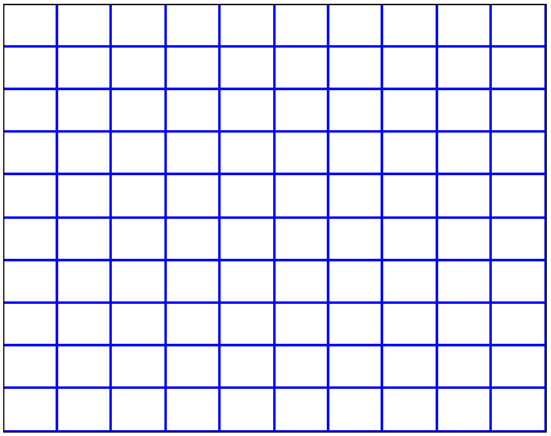
\includegraphics[width=3in]{grid1}
\end{figure}

\newpage

\vspace{5in}
\pagestyle{empty}
\begin{figure}[h!]
\centering
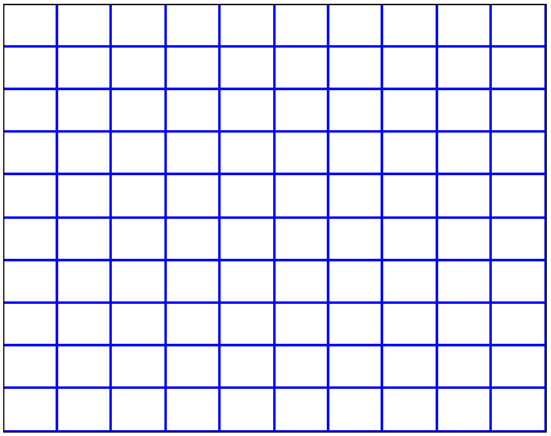
\includegraphics[width=3in]{grid1}
\end{figure}


\newpage

\vspace{5in}
\pagestyle{empty}
\begin{figure}[h!]
\centering
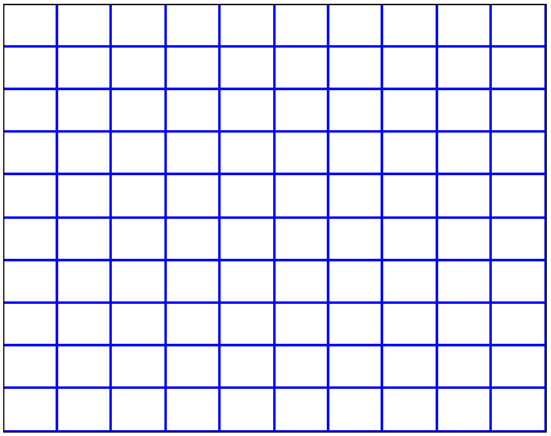
\includegraphics[width=3in]{grid1}
\end{figure}

\newpage

\vspace{5in}
\pagestyle{empty}
\begin{figure}[h!]
\centering
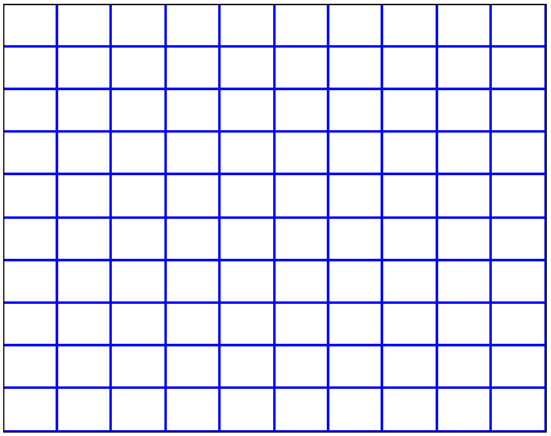
\includegraphics[width=3in]{grid1}
\end{figure}


\newpage

\vspace{5in}
\pagestyle{empty}
\begin{figure}[h!]
\centering
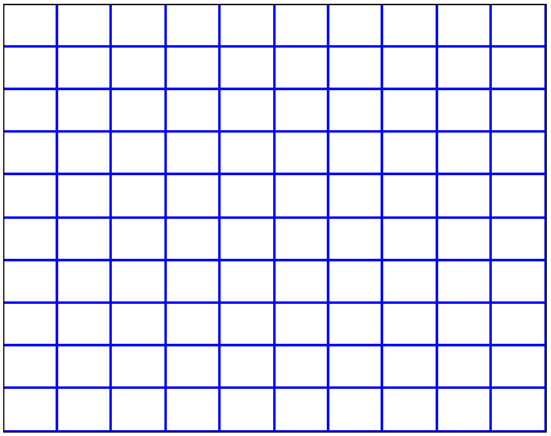
\includegraphics[width=3in]{grid1}
\end{figure}

\newpage

\vspace{5in}
\pagestyle{empty}
\begin{figure}[h!]
\centering
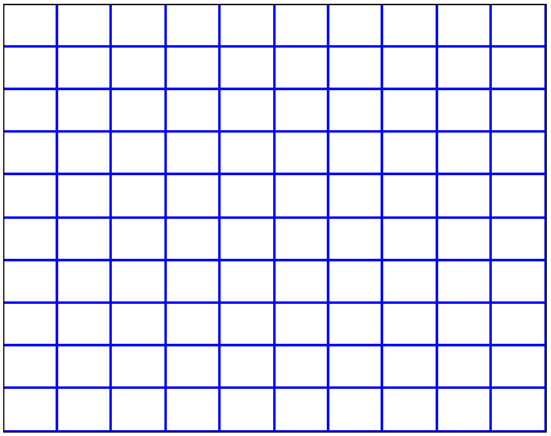
\includegraphics[width=3in]{grid1}
\end{figure}


\newpage

\vspace{5in}
\pagestyle{empty}
\begin{figure}[h!]
\centering
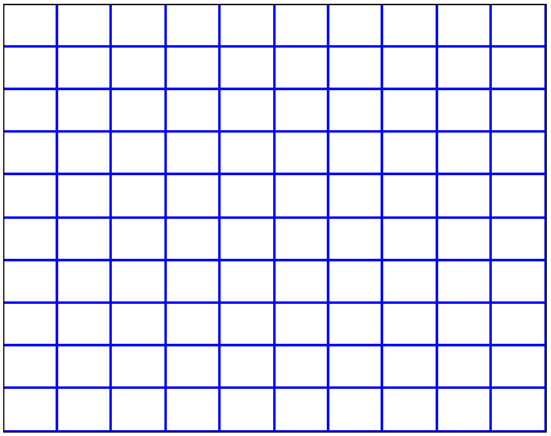
\includegraphics[width=3in]{grid1}
\end{figure}

\newpage

\vspace{5in}
\pagestyle{empty}
\begin{figure}[h!]
\centering
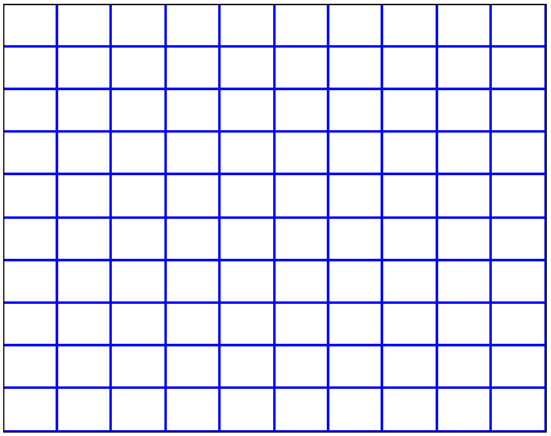
\includegraphics[width=3in]{grid1}
\end{figure}


\newpage

\vspace{5in}
\pagestyle{empty}
\begin{figure}[h!]
\centering
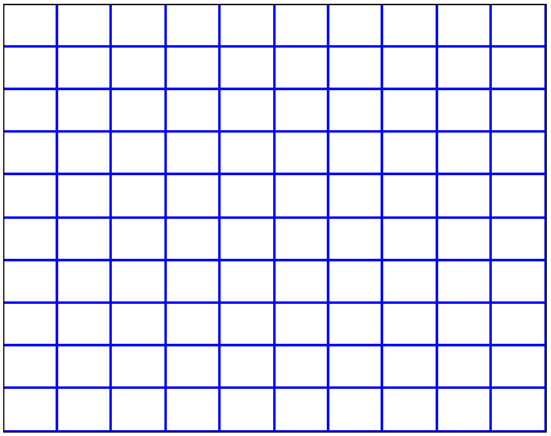
\includegraphics[width=3in]{grid1}
\end{figure}

\newpage

\vspace{5in}
\pagestyle{empty}
\begin{figure}[h!]
\centering
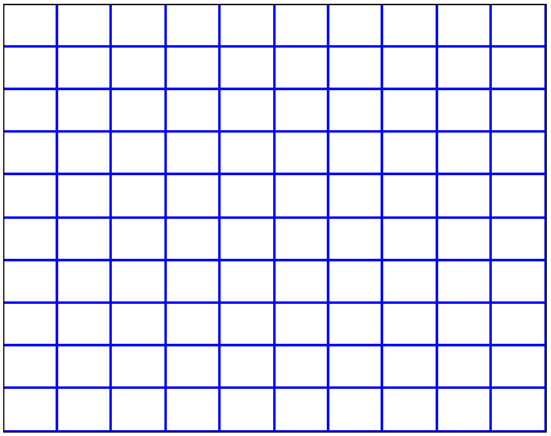
\includegraphics[width=3in]{grid1}
\end{figure}



\end{document}
